\subsection*{Kategorisering af KOL-patienter} \label{sec:kategorisering}
KOL-patienter skal have en individuel kategorisering, dette er nødvendigt for således at sikre patienter får en træning tilpasset til deres niveau. Kategoriseringen fortages første gang brugeren logger ind, som vist af \autoref{fig:logind. 
Kategoriseringen inddeler brugerne i A, B, C eller D, som beskrevet i \autoref{sec:klassifikation}. Af \autoref{fig:Kate} ses aktivitetsdiagrammet for kategoriseringen.

\begin{figure} [H]
\centering
\textbf{Aktivitetsdiagram: Kategorisering af KOL-patienter}\par\medskip
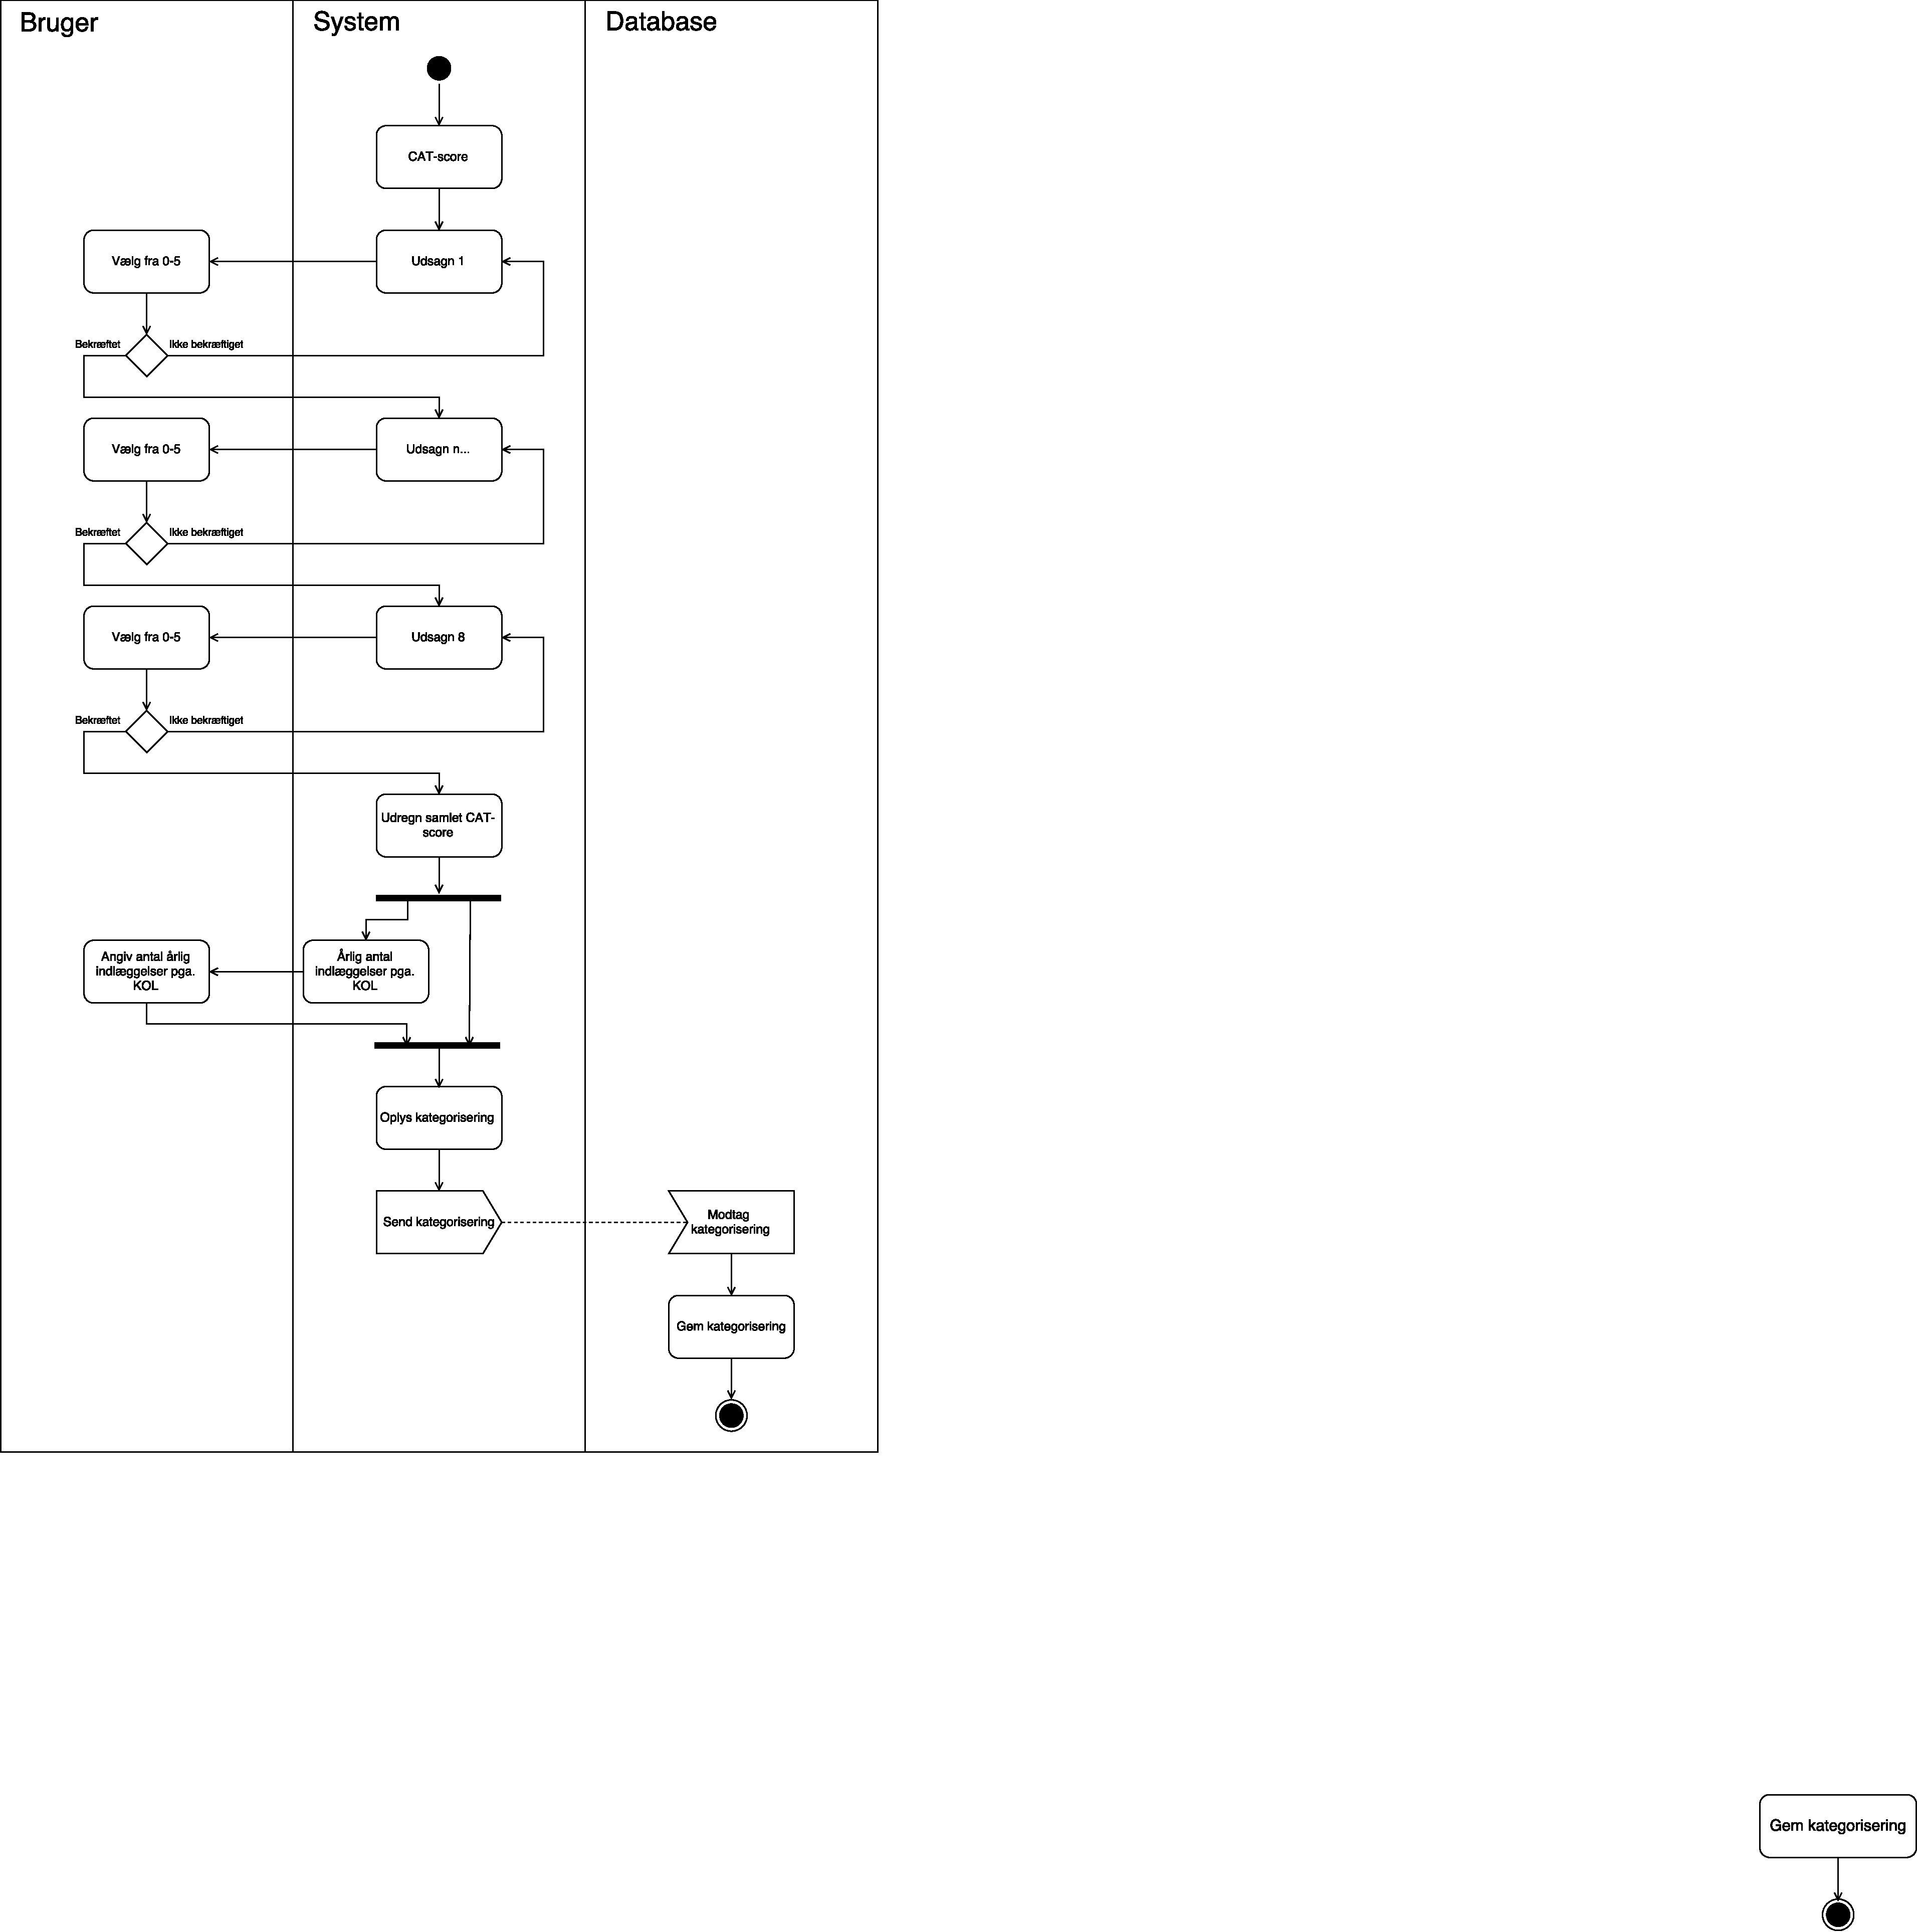
\includegraphics[width=0.65\textwidth]{figures/aktivitetsdiagram/Kategorisering}
\caption{Aktivitetsdiagram for kategorisering af KOL-patienter.}
\label{fig:Kate}
\end{figure}

\noindent
Systemet starter med at vise en grænseflade for de otte udsagn der udgør CAT, jf. \autoref{fig:CAT}. Til hvert af udsagnene angiver brugeren således en score passende til deres sygdomstilstand, hvor systemet ud fra de individuelle score udregner en samlet CAT-score. 
Dernæst vises grænsefladen for årlig antal indlæggelser på grund af KOL, hvor bruger skal angiv en passende værdi. 
Ud fra den samlede CAT-score og antal indlæggelser, udregner systemet brugers kategorisering af KOL, og viser den efterfølgende. Kategoriseringen sendes til en database for at informationen er ajourført.